\documentclass[11pt,a4paper]{article}
\usepackage[dvips]{graphicx}
\author{Alessandro Bonazzi}
\title{Neural Network for Bayesfor}
\begin{document}
\maketitle

We consider the problem of predicting the variable $y$ when the predictor
variable $x$ is known.
The easiest case will be a linear regression, but we can generalize the problem finding a solution for a statistical model of this form:
\begin{eqnarray}
     y_l = \sigma_l ( \sum_{k=1}^L w_{2kl}  \sigma_k ( \sum^K_{j=1} w_{1jk} x_j + \theta_j ) + \theta_k ) 
\end{eqnarray}

In this example we fit a neural network with 10 hidden layer a single outer layer. In other words, we find a solution for $y$ based only on the knowledge of a single variable x.

The technique used is a sequential Monte Carlo method.
You can find the documentation and the original matlab code at this address:


http://www.cs.ubc.ca/\%7Enando/software.html


Figure 1 shows the time series of the predictor variable and the true $y$.
Figure 2 shows the one-step forecast of $y$ based on $x$ and the forecast error.

\begin{figure} \includegraphics[width=12cm]{problem.eps}
\caption{Up panel: predictor $x$ time series. Low panel: target variable}
\end{figure}


\begin{figure} \includegraphics[width=12cm]{prediction.eps}
\caption{Up panel: One step forecast. Middle panel: true $y$. Low panel: error}
\end{figure}

\end{document}
